\chapter{The Best Financial Decision That Was Not Quite Theirs}

This chapter follows a short School of Hard Knocks entrepreneurship interview curated by LazyingArt LLC for Video2Book. The spoken episode is compact, but the business logic is sharp: the speaker begins with the broad answer, investing in himself, then turns to a founding story in which a venture capital rejection became useful in hindsight. There is no validated blackboard or diagram evidence for this lecture, so the displayed mathematics is not copied from a board. It is a cautious decision language for the mechanism stated in the transcript: capital can accelerate growth, but the process of getting it can consume attention.

\section{The Opening Question}

The interview begins with the cleanest possible prompt: what was the best financial decision you ever made? The first answer is not a deal, a security, or a financing structure. It is investing in oneself.

That answer gives us the outer frame. A financial decision is not only an allocation of cash. It can also be an allocation of time, judgment, skill, and attention. Then the speaker immediately narrows the frame. He moves from the general answer to a founding story involving himself and his partner.

The important sentence is paradoxical: the best decision was not really their decision, but in a sense it was. We should keep that tension in view. The venture firm made the formal decision to pass. The founders made the prior decision to seek capital, spend attention on the process, and later interpret the rejection.

\section{A Profitable Company Looking For Speed}

The company was already in a strong operating position. The transcript says it was growing fast and profitable. We can record that condition in a deliberately minimal way:
\begin{equation}
\Pi > 0 .
\end{equation}
Here \(\Pi\) denotes operating profit only in the modest sense needed for the story. It does not stand for a known profit margin, a valuation, or a full financial model.

That initial condition matters. The company was not described as searching for rescue money. The founders believed additional capital would let them expand faster. So the motive was closer to
\begin{equation}
K_{\mathrm{outside}} \longrightarrow \hbox{faster expansion}
\end{equation}
than to
\begin{equation}
K_{\mathrm{outside}} \longrightarrow \hbox{survival}.
\end{equation}
Once we see that distinction, the decision becomes more delicate. Survival financing can be forced by necessity. Acceleration financing must be compared with its costs.

\begin{definition}
Let \(K_{\mathrm{outside}}\) denote outside capital, specifically venture capital in this interview. Let \(A_{\mathrm{growth}}\) denote the expected acceleration from raising that capital, and let \(C_{\mathrm{attention}}\) denote the founder attention, energy, and focus consumed by the fundraising process.
\end{definition}

The transcript directly supports \(A_{\mathrm{growth}}\) and \(C_{\mathrm{attention}}\): the founders wanted to expand faster, and they spent a lot of energy working with the firm.

\section{The Venture Capital Courtship}

The speaker describes venture capital as a courtship. That word is doing real work. A courtship is not merely a transaction price. It is a process: meetings, persuasion, follow-up, uncertainty, waiting, and repeated attention.

We can write the broad outside-capital decision as a reconstructed accounting identity:
\begin{equation}
V_{\mathrm{net}}
\approx
A_{\mathrm{growth}}
-
C_{\mathrm{attention}}
-
C_{\mathrm{control}}
-
C_{\mathrm{dilution}} .
\end{equation}
Only the first two terms are directly grounded in the transcript. The control and dilution terms are standard entrepreneurial concerns, but the interview excerpt does not give terms, valuation, ownership percentages, or governance details. They belong in the model only as cautious reminders.

For this lecture's local point, the cleaner expression is the process value:
\begin{equation}
V_{\mathrm{process}}
=
A_{\mathrm{growth}}
-
C_{\mathrm{attention}} .
\end{equation}
Before a term sheet exists, before dilution is even quantified, the fundraising process can already be positive or negative.

\begin{figure}
\centering
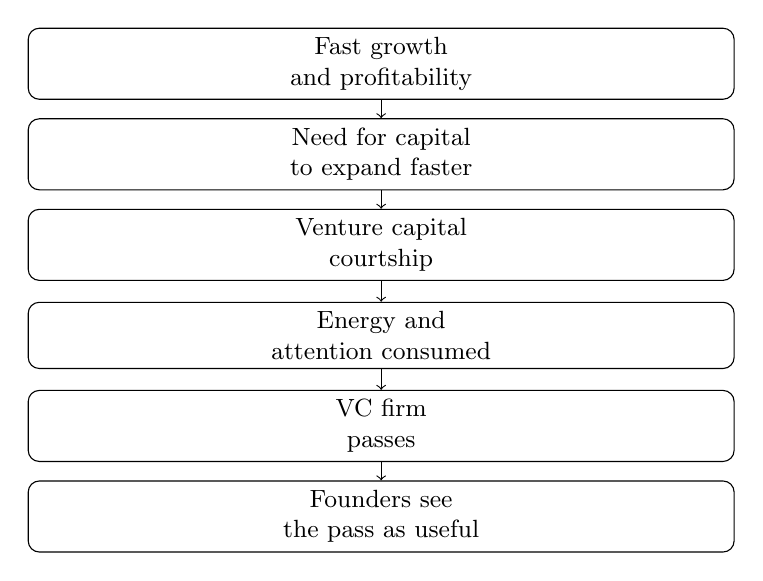
\begin{tikzpicture}[x=1cm,y=1cm, font=\small]
\node[draw, rounded corners, align=center, text width=.72\linewidth, minimum height=.72cm] (a) at (0,0) {Fast growth\\and profitability};
\node[draw, rounded corners, align=center, text width=.72\linewidth, minimum height=.72cm] (b) at (0,-1.15) {Need for capital\\to expand faster};
\node[draw, rounded corners, align=center, text width=.72\linewidth, minimum height=.72cm] (c) at (0,-2.30) {Venture capital\\courtship};
\node[draw, rounded corners, align=center, text width=.72\linewidth, minimum height=.72cm] (d) at (0,-3.45) {Energy and\\attention consumed};
\node[draw, rounded corners, align=center, text width=.72\linewidth, minimum height=.72cm] (e) at (0,-4.60) {VC firm\\passes};
\node[draw, rounded corners, align=center, text width=.72\linewidth, minimum height=.72cm] (f) at (0,-5.75) {Founders see\\the pass as useful};
\draw[->] (a) -- (b);
\draw[->] (b) -- (c);
\draw[->] (c) -- (d);
\draw[->] (d) -- (e);
\draw[->] (e) -- (f);
\end{tikzpicture}
\caption{The transcript's sequence as a narrow decision flow: profitable growth led to a search for speed, but the fundraising process exposed an attention cost.}
\end{figure}

\subsection{Question \& Answer}

\paragraph{Question.}
If the founders wanted capital to expand faster, why did the venture firm's rejection become part of the best financial decision?

\paragraph{Answer.}
Because the process revealed a cost that was easy to underestimate. The founders were not only evaluating capital. They were spending attention. The attempted raise became evidence that outside money can demand founder energy before it delivers growth.

The decision test is therefore:
\begin{equation}
\hbox{continue pursuing outside capital only if}
\qquad
V_{\mathrm{process}} > 0 .
\end{equation}
In the story, the firm passed, and the founders were relieved. The pass was not their choice in the narrow procedural sense. But the lesson was theirs: the company still had growth, profit, and focus, while the fundraising process had become frustrating.

\section{A Worked Process Calculation}

The transcript gives no numerical inputs, so the following is not a reconstruction of the company's actual finances. It is a small calculation that makes the spoken mechanism explicit.

Suppose the value of a successful financing round is \(A_{\mathrm{growth}}\), but the probability that the courtship produces a useful deal is \(p_{\mathrm{deal}}\). The expected process value is then
\begin{align}
V_{\mathrm{process}}
&=
p_{\mathrm{deal}}A_{\mathrm{growth}}
-
C_{\mathrm{attention}} .
\end{align}
The process is worth continuing only while
\begin{align}
p_{\mathrm{deal}}A_{\mathrm{growth}}
&>
C_{\mathrm{attention}} .
\end{align}
This is the simplest way to capture the lecture's reversal. As a courtship drags on, the expected value can move in two directions at once:
\begin{align}
p_{\mathrm{deal}} &\downarrow,\\
C_{\mathrm{attention}} &\uparrow.
\end{align}
The founders may begin with the thought that capital equals speed. But after enough meetings and frustration, the actual process can look like
\begin{align}
p_{\mathrm{deal}}A_{\mathrm{growth}}
-
C_{\mathrm{attention}}
&< 0 .
\end{align}
At that point, a rejection can preserve something valuable. It can stop a negative process before it consumes more of the founders' operating attention.

\section{The Decision That Was Not Fully Theirs}

We can now return to the sentence that gives the story its shape: the best decision was not really their decision, but it kind of was. The venture firm made the visible decision. It passed. But the founders had already made a sequence of decisions around the process: they sought capital, invested time in the courtship, felt the cost, and then understood the pass differently than they might have at the start.

That is a useful entrepreneurial distinction. Some outcomes are chosen directly. Others arrive from outside. But founders still have to decide what the outcome means and how to redeploy attention afterward.

\begin{remark}
This is not a general argument against venture capital. The transcript supports a narrower claim: in this case, outside capital was pursued as acceleration for an already profitable company, and the process itself became costly enough that the rejection looked beneficial in hindsight.
\end{remark}

\section{Summary}

The chapter begins with self-investment and then sharpens into a capital-allocation lesson. A profitable, fast-growing company wanted outside money to expand faster. The founders entered a venture capital courtship, spent energy on it, and were passed over. Instead of treating the rejection as pure loss, they later recognized that the process had exposed an attention cost.

The durable principle is the net view of capital:
\begin{equation}
V_{\mathrm{net}}
\approx
\hbox{growth gained}
-
\hbox{attention spent}
-
\hbox{other capital costs}.
\end{equation}
In this interview, the important financial object was not just \(K_{\mathrm{outside}}\). It was the value of capital after the hidden cost of pursuing it was counted.